\documentclass[Arkitektur/System_main.tex]{subfiles}
\begin{document}
\subsubsection{Søgning efter biler til leje}
Når en lejer ønsker at leje en bil, så skal han søge efter en i applikationens katalog, hvor udlejer har sat dem til leje. Søgningsprocesen er først beskrevet med et sekvensdiagram, hvor man ser hvordan bruger, CarnGo , samt databasen spiller sammen for at søgningsprocessen fuldføres. Dette diagram ses på figur \ref{fig:SearchProcessSD}. 
\begin{figure}[H]
    \centering
    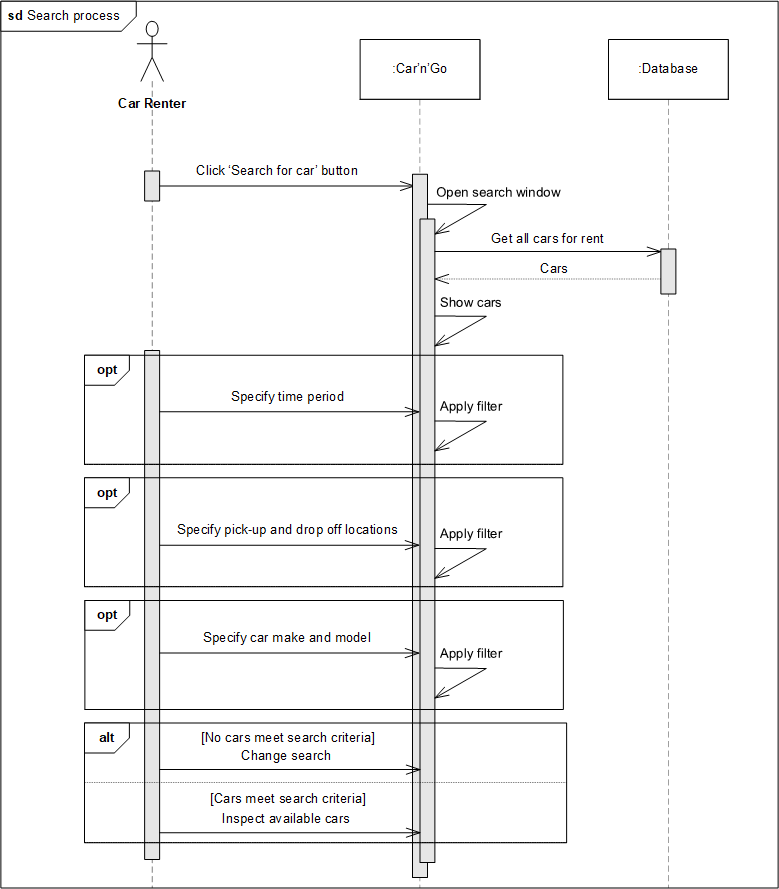
\includegraphics[width=1\textwidth]{Arkitektur/Softwarearkitektur/Searching/graphics/Search_Process_SD.png}
    \caption{Sekvensdiagram for søgning efter biler til leje. }
    \label{fig:SearchProcessSD}
\end{figure}
Der blev også lavet en applikationsmodel bestående af et klassediagram, som ses på figur \ref{fig:SearchProcessCD}, og et statemachine diagram, der ses på figur \ref{fig:SearchProcessSTM}.
\begin{figure}[H]
    \centering
    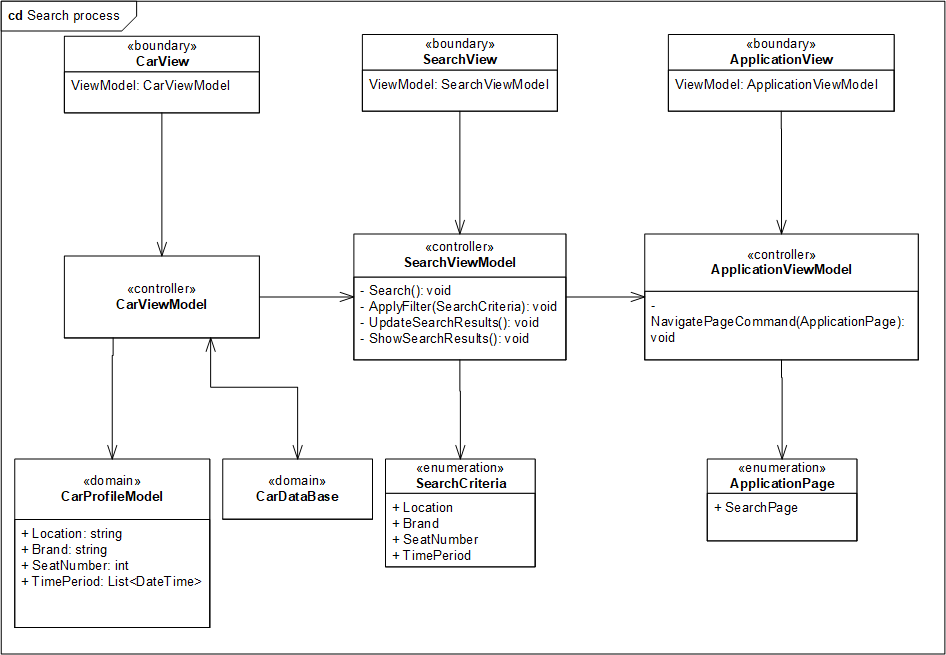
\includegraphics[width=1\textwidth]{Arkitektur/Softwarearkitektur/Searching/graphics/SearchProcessCD.png}
    \caption{Klassediagram for søgning efter biler til leje. }
    \label{fig:SearchProcessCD}
\end{figure}

\begin{figure}[H]
    \centering
    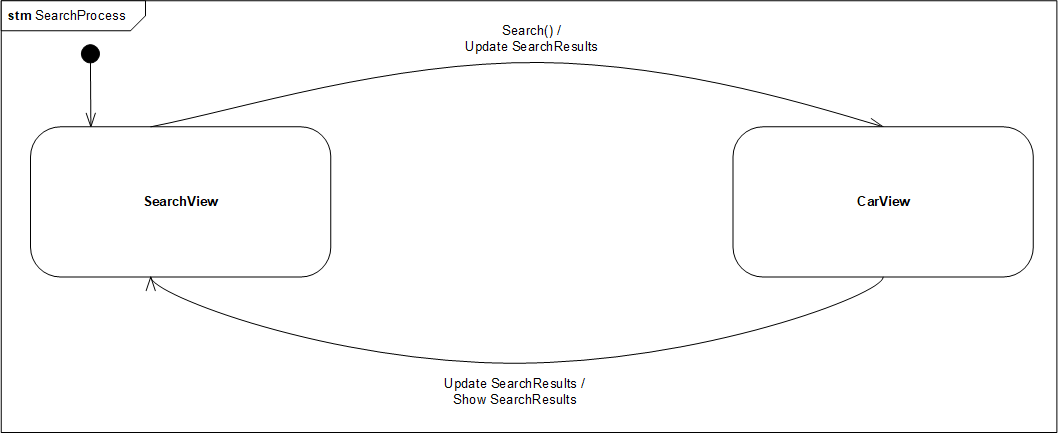
\includegraphics[width=1\textwidth]{Arkitektur/Softwarearkitektur/Searching/graphics/SearchProcessSTM.png}
    \caption{Statemachine for søgning efter biler til leje. }
    \label{fig:SearchProcessSTM}
\end{figure}


\end{document}